
To build any project, we should start with a clear understanding of what logical targets are going to be created in it. In this case, we'll follow the structure shown in Figure 12.2:

\begin{center}
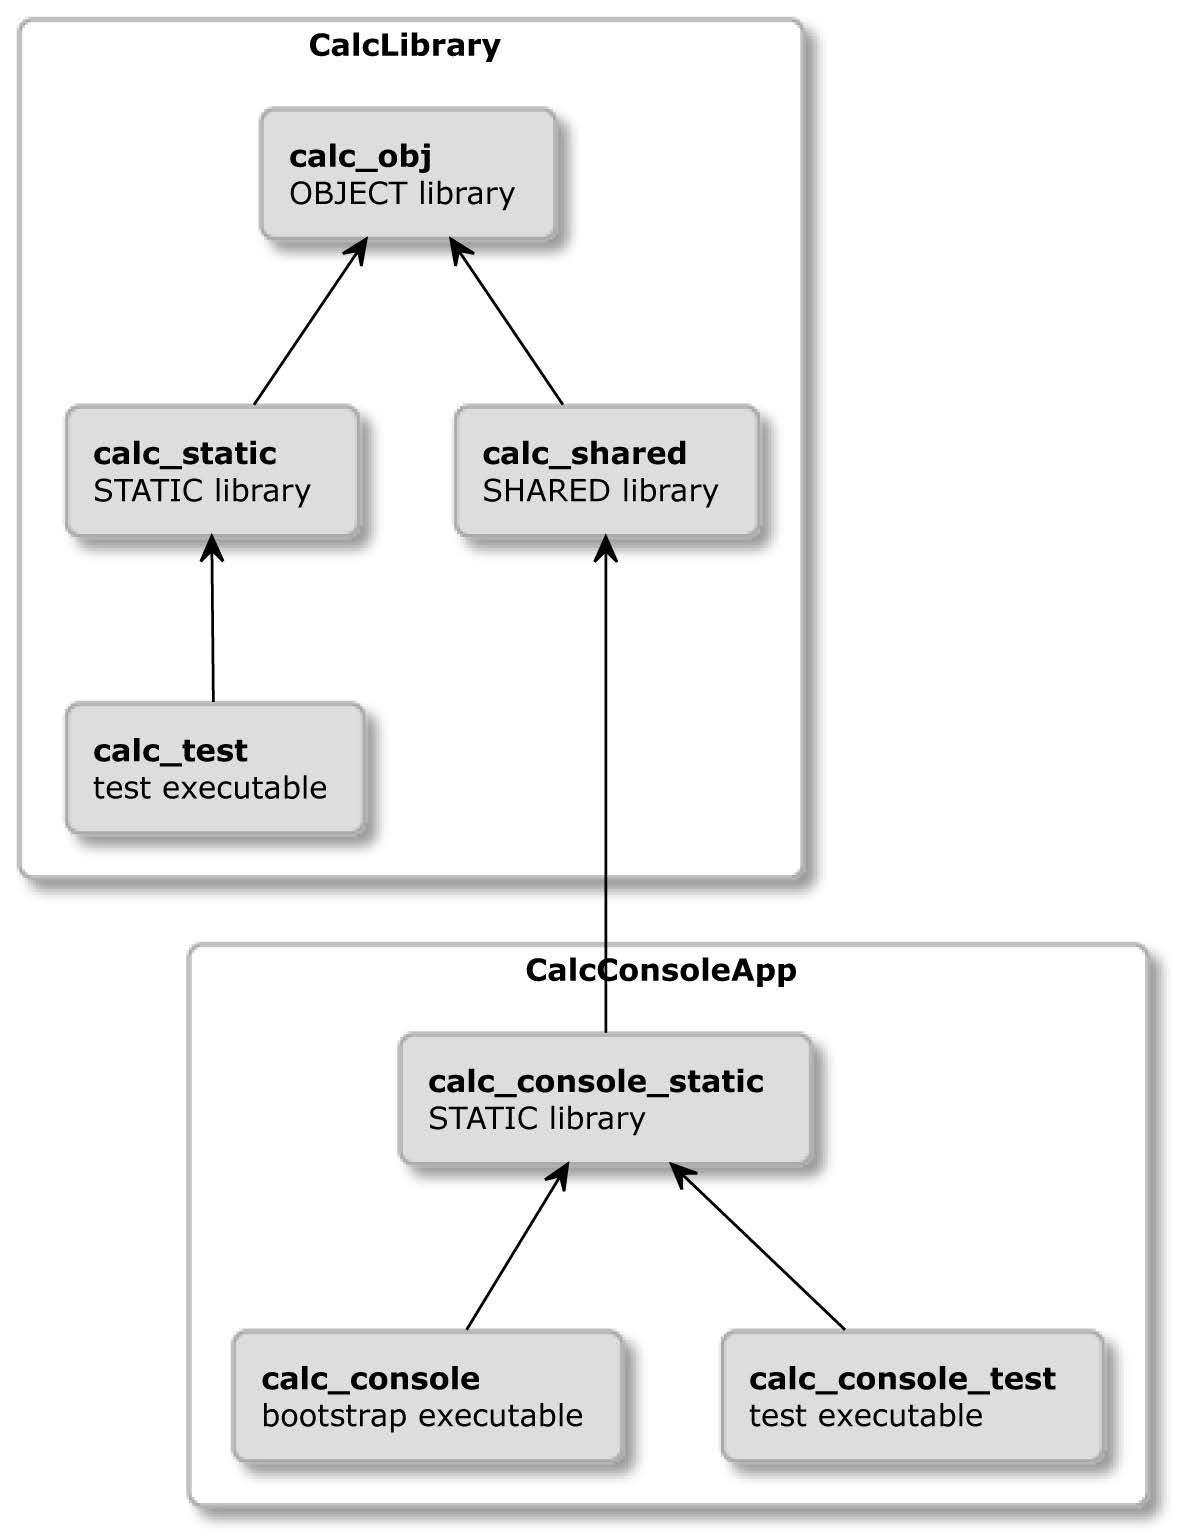
\includegraphics[width=0.8\textwidth]{content/3/chapter12/images/2.jpg}\\
Figure 12.2 – A structure of logical targets
\end{center}

Let's explore the structure by following the build order. First, we'll compile calc\_obj, which is an object library. We did mention object libraries a few times in the book, but we didn't actually introduce them as a concept. Let's do this now.

\subsubsubsection{12.3.1\hspace{0.2cm}Object libraries}

Object libraries are used to group multiple source files under a single logical target and are compiled into the (.o) object files during a build. To create an object library, we use the same method as with other libraries with the OBJECT keyword:

\begin{lstlisting}[style=styleCMake]
add_library(<target> OBJECT <sources>)
\end{lstlisting}

Object files produced during the build can be added as compiled elements to other targets with the \$<TARGET\_OBJECTS:objlib> generator expression:

\begin{lstlisting}[style=styleCMake]
add_library(... $<TARGET_OBJECTS:objlib> ...)
add_executable(... $<TARGET_OBJECTS:objlib> ...)
\end{lstlisting}

Alternatively, you can add them as dependencies with the target\_link\_libraries() command.

In our Calc library, object libraries will be useful to avoid repeating the compilation of library sources for the static and shared versions of the library. We'll just need to remember to explicitly compile the object files with POSITION\_INDEPENDENT\_CODE, as this is a requirement for a shared library.

With this out of the way, let's get back to the targets of this project: calc\_obj will provide compiled object files, which then will be used for both the calc\_static and calc\_shared libraries. What are the practical differences between them and why provide two libraries at all?

\subsubsubsection{12.3.2\hspace{0.2cm}Shared libraries versus static libraries}

We briefly introduced both types of libraries in Chapter 6, Linking with CMake. We then mentioned that overall memory usage can be better for multiple programs using the same shared library and that it's likely that a user already has the most popular libraries or knows how to quickly install them. More importantly, shared libraries are delivered in separate files that must be installed in specific paths for the dynamic linker to find them, while static libraries are merged as part of the executable file. In that form, they are slightly faster to use, as no additional lookups are required to find the location of code in memory.

As library authors, we can decide whether we're providing a static or shared version of the library, or we can simply ship both versions and leave this decision to the programmer using our library. We're opting for the latter here (just to see how it's done).

A static library will be consumed by the calc\_test target, which will contain unit tests that guarantee that the provided business functionality of the library works as expected. As mentioned, we're building both versions from the same set of compiled object files. In this scenario, it's perfectly fine to test either version, as there really should be no practical difference in their behavior.

The console app provided with calc\_console\_static target will use the shared library. This target will also link against an external dependency: the Functional Terminal (X) User Interface (FTXUI) library by Arthur Sonzogni (there is a link to the GitHub project in the Further reading section). It provides a dependence-free, cross-platform framework for text user interfaces.

The last two targets are calc\_console and calc\_console\_test. The calc\_console target is just a bootstrap main() wrapper around calc\_console\_static. Its only purpose is to extract the entry point from the business code. This allows us to write the unit tests (which need to provide their own entry point) and run them from calc\_console\_test.

We now know what targets need to be built and how they relate to each other. Let's figure out how to structure the project with files and directories.

\subsubsubsection{12.3.3\hspace{0.2cm}Project file structure}

The project consists of two primary targets, the calc library and the calc\_console executable, each of which will reside in directory trees under src and test to separate production code from tests (shown in Figure 12.3). Additionally, we'll have our files in two other directories:

\begin{itemize}
\item 
The root directory containing top-level configuration and key project documentation files

\item 
The cmake directory for all the utility modules and helper files used by CMake to build and install the project:

\begin{center}
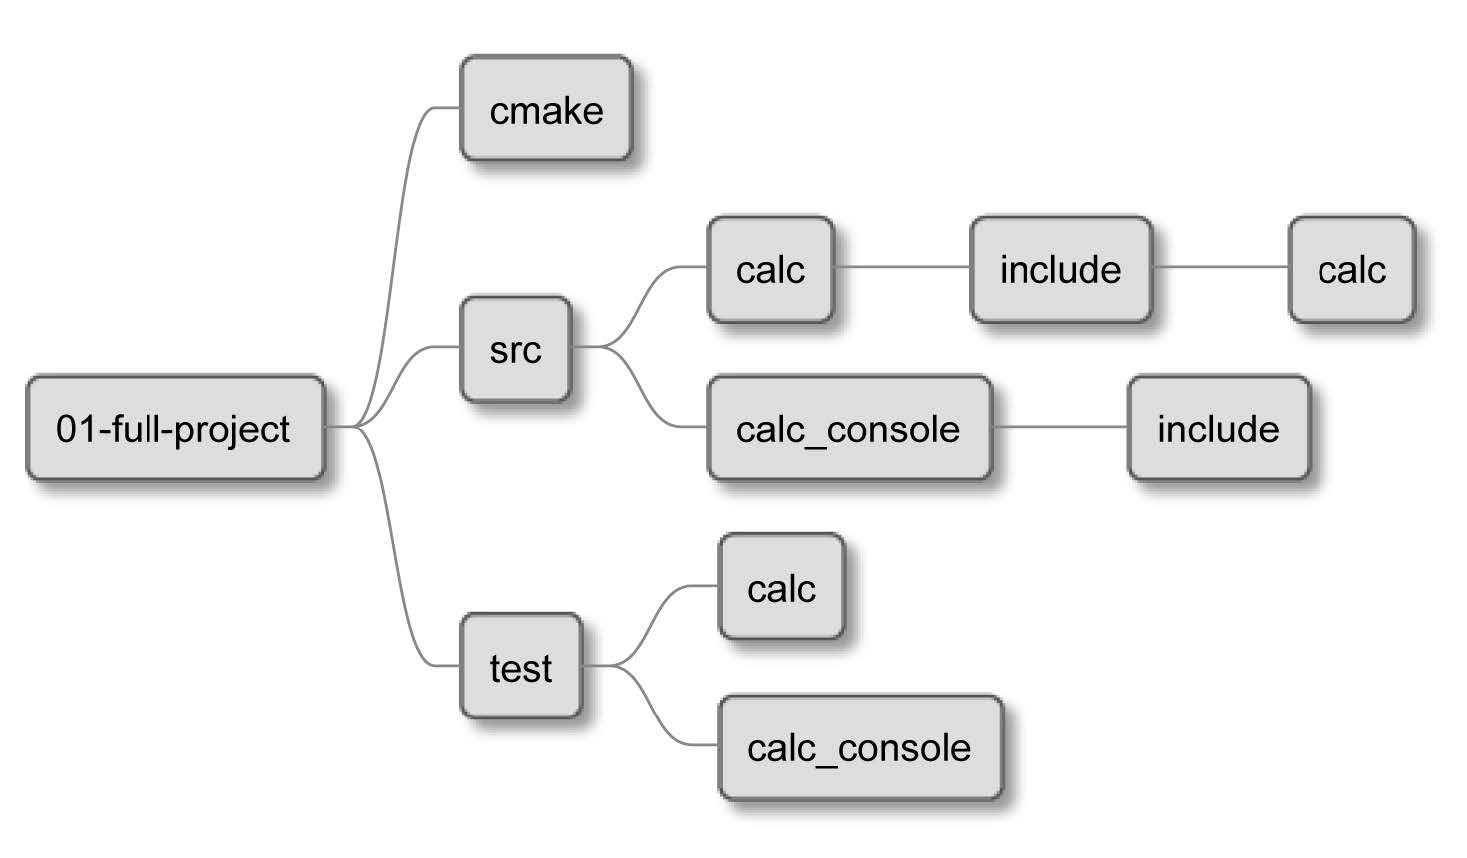
\includegraphics[width=0.8\textwidth]{content/3/chapter12/images/3.jpg}\\
Figure 12.3 – The directory structure of the project
\end{center}
\end{itemize}

Here's the full list of files in each of the four main directories:

\begin{table}[H]
	\centering
	\begin{tabular}{|l|l|}
		\hline
		\textbf{./}    & \textbf{./test}  \\ \hline
		\begin{tabular}[c]{@{}l@{}}CHANGELOG\\ CMakeLists.txt\\ CalcConfig.cmake\\ INSTALL\\ LICENSE\\ README.md\end{tabular} &
		\begin{tabular}[c]{@{}l@{}}CMakeLists.txt\\ calc/CMakeLists.txt\\ calc/calc\_test.cpp\\ calc\_console/CMakeLists.txt\\ calc\_console/tui\_test.cpp\end{tabular} \\ \hline
		\textbf{./src} & \textbf{./cmake} \\ \hline
		\begin{tabular}[c]{@{}l@{}}CMakeLists.txt\\ calc/CMakeLists.txt\\ calc/calc.cpp\\ calc/include/calc/calc.h\\ calc\_console/CMakeLists.txt\\ calc\_console/bootstrap.cpp\\ calc\_console/include/tui.h\\ calc\_console/tui.cpp\end{tabular} &
		\begin{tabular}[c]{@{}l@{}}buildinfo.h.in\\ BuildInfo.cmake\\ Coverage.cmake\\ CppCheck.cmkae\\ Doxygen.cmake\\ Format.cmake\\ GetFTXUI.cmake\\ Install.cmake\\ Memcheck.cmake\\ NoInSourceBuilds.cmake\\ Testing.cmake\end{tabular} \\ \hline
	\end{tabular}
\end{table}

Initially, the cmake directory is busier than the business code, but this will quickly change as the project grows in functionality. The effort to start a clean project is significant, but don't worry – it will pay off very soon.

We'll go through all files and see in detail what they do and what role they play in the project. This will happen in four steps: building, testing, installing and providing documentation.















